\documentclass{../download/tPRS2e}

\usepackage{epstopdf}% To incorporate .eps illustrations using PDFLaTeX, etc.
\usepackage{subfigure}% Support for small, `sub' figures and tables

\graphicspath{{media/}}

\begin{document}

\title{About some types of constraints in problems of routing}

\author{
\name{
Petunin A.A.\textsuperscript{a},
Polishuk E.G.\textsuperscript{a},
Chentsov A.G.\textsuperscript{b}\textsuperscript{a},
Chentsov P.A.\textsuperscript{a}\textsuperscript{b},
Ukolov S.S.\textsuperscript{a}$^{\ast}$\thanks{$^\ast$Corresponding author. Email: s.s.ukolov@urfu.ru}
}
\affil{\textsuperscript{a}Ural Federal University, Yekaterinburg, Russia;
\textsuperscript{b}Institute of Mathematics and Mechanics, Ural Branch of the Russian Academy of Sciences, Yekaterinburg, Russia}
}

\maketitle

\begin{abstract}
Many routing problems arising in different applications can be interpreted as a discrete optimization problem with additional constraints. The latter include generalized travelling salesman problem (GTSP), to which task of tool routing for CNC thermal cutting machines is sometimes reduced. Technological requirements bound to thermal fields distribution during cutting process are of great importance when developing algorithms for this task solution. These requirements give rise to some specific constraints for GTSP. This paper provides a mathematical formulation for the problem of thermal fields calculating during metal sheet thermal cutting. Corresponding algorithm with its programmatic implementation is considered. The mathematical model allowing taking such constraints into account considering other routing problems is discussed either. \end{abstract}

\begin{keywords}
thermal cutting;
discrete optimization;
toolpath routing;
technological constraints;
dynamic programming;
thermal deformations
\end{keywords}

\section{Introduction}

In various industries many parts are produced from sheet materials by CNC equipment.
Such kind of equipment includes, for instance, machines for laser, plasma, gas, and water-jet cutting.
Special software (Computer-Aided Manufacturing, CAM systems) provides an automation of development of NC (numerical control) programs.
Generating of NC programs is next step after nesting that is positioning parts onto sheet material.
Optimization of sheet utilization reduces the cost of sheet material used for parts producing.
The nesting problem is not considered in this study.
The control programs contain information about tool path for CNC machine and some technological commands.
Optimization of tool path reduces time and cost of cutting process.
First classification of problem was conducted by \cite{hoeft_heuristics_1997}. 
Tool path problems are usually divided into 4 classes depending on cutting technique and its parameters (see, for example, \cite{dewil_improvement_2015}):

\begin{enumerate}
\item \textit{Continuous Cutting Problem (CCP)}.
\item \textit{Endpoint Cutting Problem (ECP)}.
\item \textit{Intermittent Cutting Problem (ICP)}. 
\item \textit{Generalized Traveling Salesman Problem (GTSP)}.
\end{enumerate}

\cite{petunin_modeling_2015} offered new classification of cutting techniques and described one more class of problem:
\textit{Segment Continuous Cutting Problem (SCCP)}.

\subsection{Tool Path Components}

The tool path contains the following components (see Fig.1):

\begin{itemize}
\item Pierce points (piercings);
\item Points of switching the tool off;
\item Tool trajectory from piercing up to point of switching the tool off; 
\item Lead-in (tool trajectory from piercing up to the entry point on the equidistant contours); 
\item Lead-out (tool trajectory from exit point on equidistant contour up to tool switching off point); 
\item Airtime motions (linear movement from tool switching off point up to the next piercing).
\end{itemize}

\subsection{Cutting Techniques}

\section{Formal Definition of Tool Path}

\section{Tool Path Constraints Formalization}

\subsection{Precedence Constraint}

\subsection{Piercing Coordinates Constraints}

\begin{figure}
\begin{center}
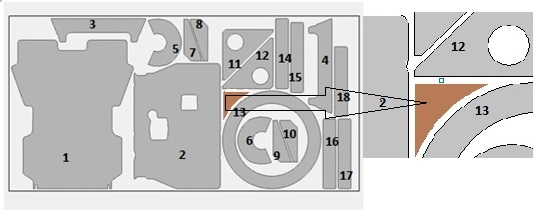
\includegraphics[width=\textwidth]{ppc.jpeg}
\caption{Feasible piercing area is marked with brown color.} \label{piercing-area}
\end{center}
\end{figure}

See Fig. \ref{piercing-area}

\subsection{Part Hardness Rule}

\subsubsection{Formalization of Part Hardness Rule}

\subsubsection{Thermal Distribution Calculations}

\subsection{Sheet Hardness Rules}

\section{Discrete Optimization Algorithms}

\begin{figure}
\begin{center}
\subfigure[Exact SCCP solution.]{
\resizebox*{0.4\textwidth}{!}{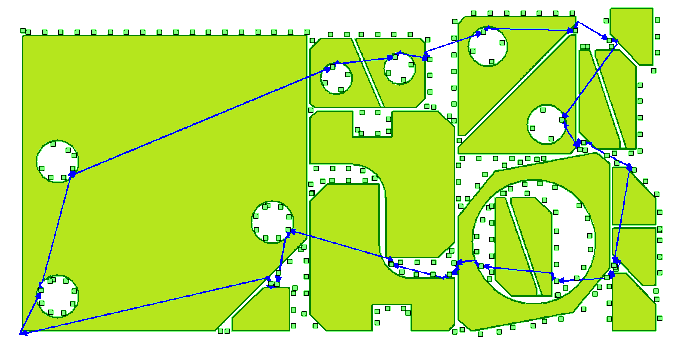
\includegraphics{nest-a.png}}}
\subfigure[Solution with thermal cutting constraints.]{
\resizebox*{0.4\textwidth}{!}{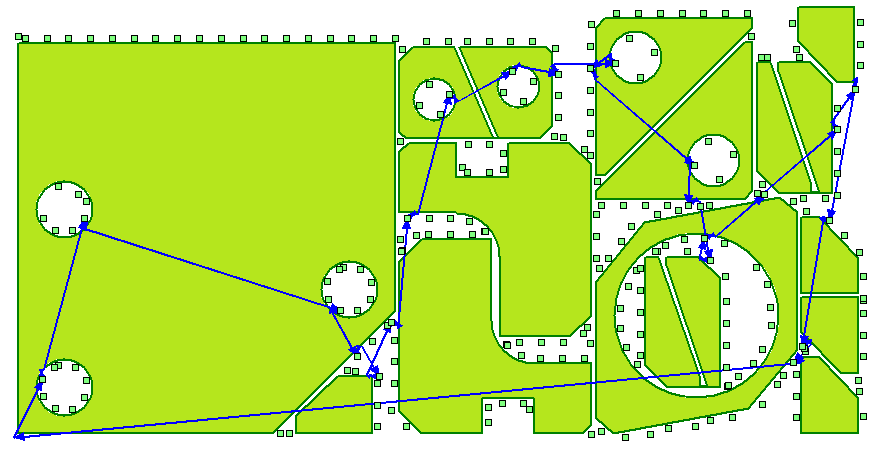
\includegraphics{nest-b.png}}}
\caption{Results of tool path optimizations.} \label{nesting-results}
\end{center}
\end{figure}

See Fig. \ref{nesting-results}...

\section*{Acknowledgements}

The work was supported by Act 211 Government of the Russian Federation, contract № 02.A03.21.0006

\bibliographystyle{../download/tPRS}
\nocite{*}
\bibliography{Investigation}



\end{document}
